% Created 2020-07-17 sex 11:46
% Intended LaTeX compiler: pdflatex
\documentclass[11pt]{article}
\usepackage[utf8]{inputenc}
\usepackage[T1]{fontenc}
\usepackage{graphicx}
\usepackage{grffile}
\usepackage{longtable}
\usepackage{wrapfig}
\usepackage{rotating}
\usepackage[normalem]{ulem}
\usepackage{amsmath}
\usepackage{textcomp}
\usepackage{amssymb}
\usepackage{capt-of}
\usepackage{hyperref}
\usepackage[margin=0.5in]{geometry}
\author{Lucas Pereira}
\date{\today}
\title{}
\hypersetup{
 pdfauthor={Lucas Pereira},
 pdftitle={},
 pdfkeywords={},
 pdfsubject={},
 pdfcreator={Emacs 26.3 (Org mode 9.1.9)}, 
 pdflang={English}}
\begin{document}

\tableofcontents


\section{MONETDB Internals}
\label{sec:orgc4fc073}

\url{http://sites.computer.org/debull/A12mar/monetdb.pdf}
\href{https://www.monetdb.org/Documentation/MonetDBInternals/Overview}{MonetDB Internals}
\href{https://www.monetdb.org/Developers/SourceCompile}{Source Compile}

Source Documentation -> monetdb\(_{\text{source}}\)/lib/monetdb5/algebra.mal

\subsection{Redesign considerations.}
\label{sec:orgbc7f831}
Redesign of the MonetDB software driven by the need to reduce the effort to extend the system into novel directions and to reduce
the \textbf{Total Execution Cost (TEC)}.

\textbf{TEC}:
\begin{itemize}
\item API message handling                (\textbf{A})
\item Parsing and semantic analysis       (\textbf{P})
\item Optimization and plan generation    (\textbf{O})
\item Data access to the persistent store (\textbf{D})
\item Execution of the query terms        (\textbf{E})
\item Result delivery to the application  (\textbf{R})
\end{itemize}

OLTP -> Online Transaction Processing -> expected most of the cost to be in (P,O)
OLAP -> Online Analytical Processing  -> expected most of the cost to be in (D,E,R)

\subsection{Storage Model}
\label{sec:org05ee127}
\begin{itemize}
\item Represents relational tables using vertical fragmentation.
\item Stores each column in a separate \{(OID,value)\} table,  called a \textbf{BAT (Binary Association Table)}
\item Relies on a low-level relational algebra called the BAT algebra, which takes BATs and scalar values as input.
\item The complete result is always stored in (intermediate) BATs, and the result of an SQL query is a collection of BATs.

\item \textbf{BAT} is implemented as an ordinary C-array. OID maps to the index in the array.
\item Persistent version of \textbf{BAT} is a \textbf{memory mapped file}.
\item \textbf{O(1) positional database lookup mechanism} (MMU - memory management unit)
\end{itemize}

\subsection{All (relational) operators exploit a small set of properties:}
\label{sec:org3c3b01a}
\begin{itemize}
\item seq       - the sequence base, a mapping from array index 0 into a OID value
\item key       - the values in the column are unique
\item nil       - there is at least one NIL value
\item nonil     - it is unknown if there NIL values
\item dense     - the numeric values in the column form a dense sequence
\item sorted    - the column contains a sorted list for ordered domains
\item revsorted - the column contains a reversed sorted list
\end{itemize}

\subsection{Execution Model}
\label{sec:org40eb6ad}
\begin{itemize}
\item \textbf{MonetDB} kernel is an abstract machine, programmed in the \textbf{MonetDB Assemblee Language (MAL)}.
\item Each relational algebra operator corresponds to a \textbf{MAL instruction} (zero degrees of freedom).
\item Each \textbf{BAT algebra operator} maps to a simple \textbf{MAL instruction}.
\end{itemize}

\subsection{Software Stack}
\label{sec:org3cc39d9}
Three software layers:
\begin{itemize}
\item \textbf{FRONT-END} \textbf{Query language parser and a heuristic, language - and data model - specific optimizer}. \textbf{OUTPUT} -> logical plan expressed in MAL.
\item \textbf{BACK-END} \textbf{Collection of optimizer modules} -> assembled into an optimization pipeline
\item \textbf{MAL interpreter} -> contains the library of highly optimized implementation of the binary relational algebra operators.
\end{itemize}


\section{Binary Association Tables}
\label{sec:orgc769f25}

\textbf{Key-Value Pair Model}

\begin{figure}[htbp]
\centering
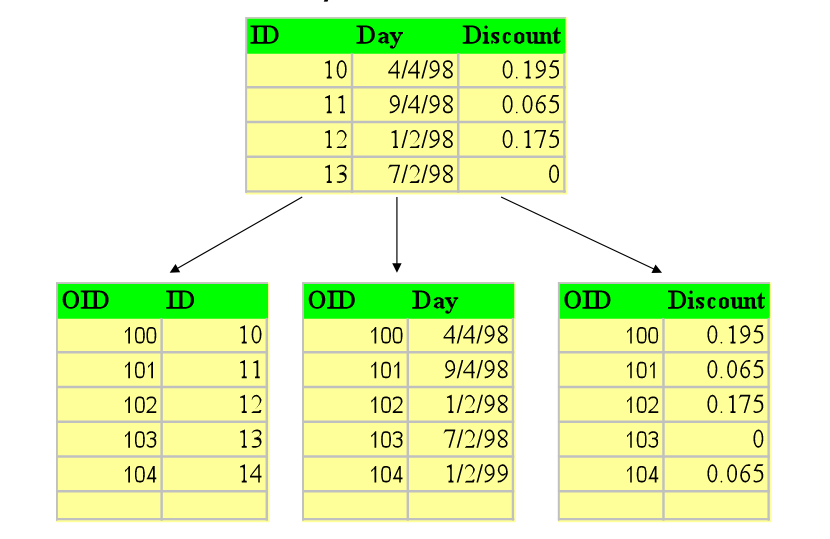
\includegraphics[width=4.0in]{./Pictures/BAT.png}
\caption{\label{fig:org86beea6}
Bat Sample}
\end{figure}

\section{MAL Reference (MonetDB Assembly Language)}
\label{sec:org30106bd}

\begin{itemize}
\item MAL program is considered a specification of intended computation and data flow behavior.
\item Language syntax uses a functional style definition of actions and mark those that affect the flow explicitly.
\end{itemize}

\subsection{Literals (follow the lexical conventions of C)}
\label{sec:org456cfcd}

\begin{center}
\begin{tabular}{lll}
\hline
\textbf{Hardwire Types} & \textbf{Temporal Types} & \textbf{IPv4 addresses and URLs}\\
\hline
bit (bit) & date & inet\\
\hline
bte (byte) & daytime & url\\
\hline
chr (char) & time & UUID\\
\hline
wrd (word) & timestamp & json\\
\hline
sht (short) & - & -\\
\hline
int (integer) & - & -\\
\hline
lng (long) & - & -\\
\hline
oid (object id) & - & -\\
\hline
flt (float) & - & -\\
\hline
dbl (double) & - & -\\
\hline
str (string) & - & -\\
\hline
\end{tabular}
\end{center}

\subsection{Variables}
\label{sec:org8adf0eb}

\textbf{User Defined} -> start with a letter
\textbf{Temporary}    -> start with X\_ (generated internally by optimizers)

\subsection{Instructions}
\label{sec:orgc2ffb0f}

\textbf{One liners}   -> easy to parse

\begin{figure}[htbp]
\centering
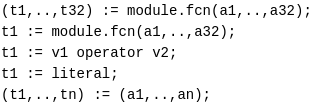
\includegraphics[width=2.0in]{./Pictures/instructions-ex.png}
\caption{\label{fig:orge799433}
Instructions example}
\end{figure}

\subsection{Type System}
\label{sec:orgc4974fd}

\textbf{Strongly typed language}

\begin{figure}[htbp]
\centering
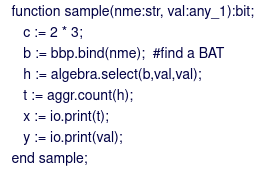
\includegraphics[width=2.0in]{./Pictures/poly-ex.png}
\caption{\label{fig:org75c537a}
Polymophism example}
\end{figure}

\begin{itemize}
\item Polymorphic given by "any".
\item Type checker (intelligent type resolution).
\end{itemize}

\subsection{Flow of Control}
\label{sec:org284973a}

\textbf{For statement implementation:}
\begin{figure}[htbp]
\centering
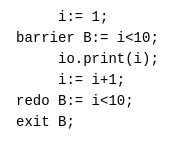
\includegraphics[width=2.0in]{./Pictures/for-ex.png}
\caption{\label{fig:org53c875f}
For example}
\end{figure}

\textbf{If statement implementation:}
\begin{figure}[htbp]
\centering
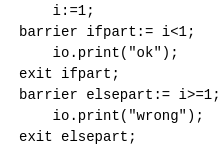
\includegraphics[width=2.0in]{./Pictures/if-ex.png}
\caption{\label{fig:org67e727c}
If example}
\end{figure}

\subsection{Exceptions}
\label{sec:org770eebf}
(\textbf{To explore.})

\subsection{Functions}
\label{sec:orgf2bcbe8}

\textbf{Function example}
\begin{figure}[htbp]
\centering
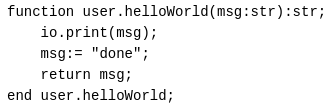
\includegraphics[width=2.0in]{./Pictures/fun-ex.png}
\caption{\label{fig:orgdb1eeef}
Function example}
\end{figure}

\textbf{Side Effects}
\begin{itemize}
\item Functions can be pre-pended with the keyword unsafe.
\item Designates that execution of the function may change the state of the database or sends information to the client.
\item Unsafe functions are critical for the optimizers -> order of execution should be guaranteed.
\item Functions that return \textbf{:void} -> unsafe by default.
\end{itemize}

\textbf{Inline Functions}
\begin{itemize}
\item Functions prepended with the keyword \textbf{inline} are a target for the optimizers to be inlined. -> reduce the function call overhead.
\end{itemize}

\subsection{MAL Syntax}
\label{sec:org002a47c}

\textbf{Expressed in extended Backus–Naur form (EBNF)} \href{https://en.wikipedia.org/wiki/Extended\_Backus\%E2\%80\%93Naur\_form}{Wiki}

\begin{center}
\begin{tabular}{ll}
\hline
Alternative constructors & (vertical bar) grouped by ()\\
\hline
Repetition & '+'-> at least once; '*'-> many\\
\hline
Lexical tokens & small capitals\\
\hline
\end{tabular}
\end{center}

\begin{figure}[htbp]
\centering
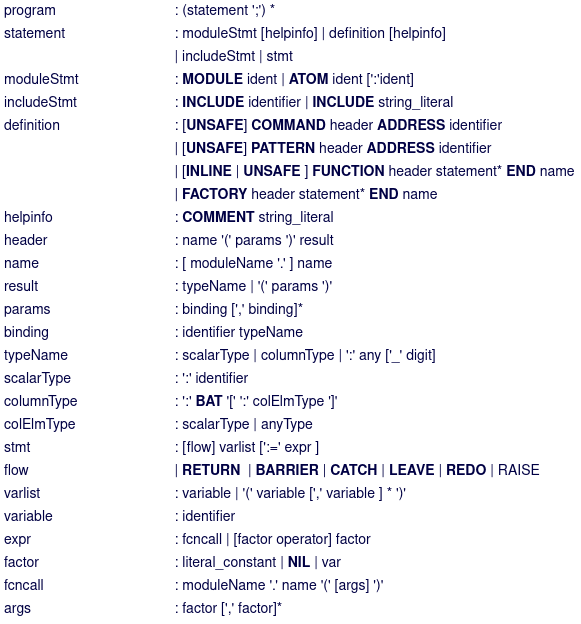
\includegraphics[width=2.0in]{./Pictures/syntax.png}
\caption{\label{fig:org2aae521}
Syntax example}
\end{figure}

\subsection{MAL Interpreter}
\label{sec:orgc70a39b}
(\textbf{To explore.})

\subsection{MAL Debugger}
\label{sec:org2e426fa}
(\textbf{To explore.})

\subsection{MAL Profiler}
\label{sec:org41867fc}

\textbf{Stethoscope REPLACED WITH Pystethoscope}

The program stethoscope is a simple Linux application that can attach itself to a running MonetDB server and extracts
the profiler events from concurrent running queries. Stethoscope is an online-only inspection tool, i.e., it only
monitors the execution state of the current queries and outputs the information in STDOUT for immediate inspection.
For example, the following command tracks the microsecond ticks for all database instructions denoted in MAL on a database called “voc”:

\$ stethoscope -u monetdb -P monetdb -d voc

Discontinued:
\begin{itemize}
\item Tachograph
\item Tomograph
\end{itemize}

\subsection{MAL Optimizers}
\label{sec:orgb48d3c8}
\textbf{Triggered by experimentation and curiousity}\\
\textbf{Check source}\\
 Cost Model, Alias Removal, Landscape, Lifespans, Macro Processing, Memoization, Multiplex Functions, Remove Actions, Stack Reduction, Garbage Collector

\subsubsection{Building Blocks}
\label{sec:org8a71914}
There are examples for a user to build a Optimizer
\subsubsection{Coercions}
\label{sec:org61b41fb}
Removes coercions that are not needed --> v:= calc.int(23);
(sloppy code-generator or function call resolution decision)

\subsubsection{Common Subexpressions}
\label{sec:org7c3c819}
\begin{figure}[htbp]
\centering
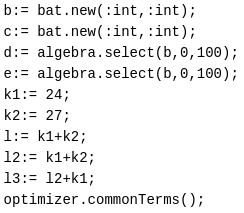
\includegraphics[width=2.0in]{./Pictures/opt-common-subs-1.png}
\caption{\label{fig:org7125cc8}
Syntax example}
\end{figure}              

\begin{figure}[htbp]
\centering
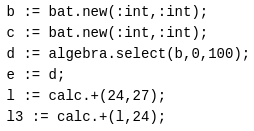
\includegraphics[width=2.0in]{./Pictures/opt-common-subs-1+.png}
\caption{\label{fig:orge7ad7c9}
Syntax example 2}
\end{figure}

\subsubsection{Constant Expression Evaluation}
\label{sec:orga210bc4}

\begin{figure}[htbp]
\centering
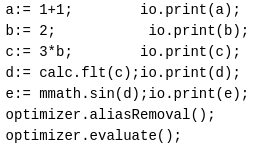
\includegraphics[width=2.0in]{./Pictures/const-exps-eval-1.png}
\caption{\label{fig:orga8c0465}
Expression example}
\end{figure}             

\begin{figure}[htbp]
\centering
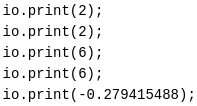
\includegraphics[width=2.0in]{./Pictures/const-exps-eval-1+.png}
\caption{\label{fig:org9bc8cbf}
Expression example 2}
\end{figure}


\subsubsection{Data Flow}
\label{sec:org4cde6d9}
Query executions without side effects can be rearranged.

\subsubsection{Join Paths}
\label{sec:org893930b}
Looks up the MAL query and "composes" multiple joins. \textbf{algebra.join -> algebra.joinPath}


\subsection{MAL Modules Overview}
\label{sec:org765af6e}
\begin{itemize}
\item Alarm
\item Algebra (Important)
\item BAT (Important)
\item BAT Extensions (Important)
\item BBP
\item Calculator
\item Clients (Important)
\item Debugger (Important)
\item Factories
\item Groups (Important)
\item I/O
\item Imprints
\item Inspect
\item Iterators
\item Language Extension
\item Logger
\item MAPI Interface (Important)
\item Manual
\item PCRE Library
\item Profiler
\item Remote
\item Transaction
\end{itemize}


\pagebreak

\section{MAL Algebra}
\label{sec:orgb0681c2}
\subsection{Misc}
\label{sec:orgf6ab7d4}
\begin{longtable}{|l|l|p{10cm}|}
\hline
MAL & Address & Comment\\
\hline
\endfirsthead
\multicolumn{3}{l}{Continued from previous page} \\
\hline

MAL & Address & Comment \\

\hline
\endhead
\hline\multicolumn{3}{r}{Continued on next page} \\
\endfoot
\endlastfoot
\hline
groupby & ALGgroupby & Produces a new BAT with groups indentified by the head column. (The result contains tail times the head value, ie the tail contains the result group sizes.)\\
\hline
find & ALGfind & Returns the index position of a value. If no such BUN exists return OID-nil.\\
\hline
fetch & ALGfetchoid & Returns the value of the BUN at x-th position with 0 <= x < b.count\\
\hline
project & ALGprojecttail & Fill the tail with a constant\\
\hline
projection & ALGprojection & Project left input onto right input.\\
\hline
projection2 & ALGprojection2 & Project left input onto right inputs which should be consecutive.\\
\hline
\end{longtable}

\subsection{BAT copying}
\label{sec:orga3236dd}
\begin{longtable}{|l|l|p{10cm}|}
\hline
MAL & Address & Comment\\
\hline
\endfirsthead
\multicolumn{3}{l}{Continued from previous page} \\
\hline

MAL & Address & Comment \\

\hline
\endhead
\hline\multicolumn{3}{r}{Continued on next page} \\
\endfoot
\endlastfoot
\hline
copy & ALGcopy & Returns physical copy of a BAT.\\
\hline
exist & ALGexist & Returns whether 'val' occurs in b.\\
\hline
\end{longtable}

\subsection{Selecting}
\label{sec:org854b937}
The range selections are targeted at the tail of the BAT.
\begin{longtable}{|l|l|p{10cm}|}
\hline
MAL & Address & Comment\\
\hline
\endfirsthead
\multicolumn{3}{l}{Continued from previous page} \\
\hline

MAL & Address & Comment \\

\hline
\endhead
\hline\multicolumn{3}{r}{Continued on next page} \\
\endfoot
\endlastfoot
\hline
select & ALGselect1 & Select all head values for which the tail value is in range.	Input is a dense-headed BAT, output is a dense-headed BAT with in	the tail the head value of the input BAT for which the tail value	is between the values low and high (inclusive if li respectively	hi is set).  The output BAT is sorted on the tail value.\\
\hline
select & ALGselect2 & Select all head values of the first input BAT for which the tail value	is in range and for which the head value occurs in the tail of the	second input BAT.	The first input is a dense-headed BAT, the second input is a	dense-headed BAT with sorted tail, output is a dense-headed BAT	with in the tail the head value of the input BAT for which the	tail value is between the values low and high (inclusive if li	respectively hi is set).  The output BAT is sorted on the tail	value.\\
\hline
select & ALGselect1nil & With unknown set, each nil != nil\\
\hline
select & ALGselect2nil & With unknown set, each nil != nil\\
\hline
selectNotNil & ALGselectNotNil & Select all not-nil values.\\
\hline
thetaselect & ALGthetaselect1 & Select all head values for which the tail value obeys the relation value OP VAL.	Input is a dense-headed BAT, output is a dense-headed BAT with in	the tail the head value of the input BAT for which the relationship holds.  The output BAT is sorted on the tail value.\\
\hline
thetaselect & ALGthetaselect2 & Select all head values of the first input BAT for which the tail value	obeys the relation value OP VAL and for which the head value occurs in	the tail of the second input BAT.	Input is a dense-headed BAT, output is a dense-headed BAT with in	the tail the head value of the input BAT for which the relationship holds.  The output BAT is sorted on the tail value.\\
\hline
\end{longtable}

\subsection{Sort}
\label{sec:org4b4c3d0}
\begin{longtable}{|l|l|p{10cm}|}
\hline
MAL & Address & Comment\\
\hline
\endfirsthead
\multicolumn{3}{l}{Continued from previous page} \\
\hline

MAL & Address & Comment \\

\hline
\endhead
\hline\multicolumn{3}{r}{Continued on next page} \\
\endfoot
\endlastfoot
\hline
sort & ALGsort11 & Returns a copy of the BAT sorted on tail values. The order is descending if the reverse bit is set. This is a stable sort if the stable bit is set.\\
\hline
sort & ALGsort12 & Returns a copy of the BAT sorted on tail values and a BAT that specifies how the input was reordered. The order is descending if the reverse bit is set. This is a stable sort if the stable bit is set.\\
\hline
sort & ALGsort13 & Returns a copy of the BAT sorted on tail values, a BAT that specifies how the input was reordered, and a BAT with group information. The order is descending if the reverse bit is set. This is a stable sort if the stable bit is set.\\
\hline
sort & ALGsort21 & Returns a copy of the BAT sorted on tail values. The order is descending if the reverse bit is set. This is a stable sort if the stable bit is set.\\
\hline
sort & ALGsort22 & Returns a copy of the BAT sorted on tail values and a BAT that specifies how the input was reordered. The order is descending if the reverse bit is set. This is a stable sort if the stable bit is set.\\
\hline
sort & ALGsort23 & Returns a copy of the BAT sorted on tail values, a BAT that specifies how the input was reordered, and a BAT with group information. The order is descending if the reverse bit is set. This is a stable sort if the stable bit is set.\\
\hline
sort & ALGsort31 & Returns a copy of the BAT sorted on tail values. The order is descending if the reverse bit is set. This is a stable sort if the stable bit is set.\\
\hline
sort & ALGsort32 & Returns a copy of the BAT sorted on tail values and a BAT that specifies how the input was reordered. The order is descending if the reverse bit is set. This is a stable sort if the stable bit is set.\\
\hline
sort & ALGsort33 & Returns a copy of the BAT sorted on tail values, a BAT that specifies how the input was reordered, and a BAT with group information. The order is descending if the reverse bit is set. This is a stable sort if the stable bit is set.\\
\hline
\end{longtable}

\subsection{Unique}
\label{sec:org3517f5b}
\begin{longtable}{|l|l|p{10cm}|}
\hline
MAL & Address & Comment\\
\hline
\endfirsthead
\multicolumn{3}{l}{Continued from previous page} \\
\hline

MAL & Address & Comment \\

\hline
\endhead
\hline\multicolumn{3}{r}{Continued on next page} \\
\endfoot
\endlastfoot
\hline
unique & ALGunique2 & Select all unique values from the tail of the first input. Input is a dense-headed BAT, the second input is a	dense-headed BAT with sorted tail, output is a dense-headed	BAT with in the tail the head value of the input BAT that was	selected.  The output BAT is sorted on the tail value.  The	second input BAT is a list of candidates.\\
\hline
unique & ALGunique1 & Select all unique values from the tail of the input. Input is a dense-headed BAT, output is a dense-headed BAT with	in the tail the head value of the input BAT that was selected.	The output BAT is sorted on the tail value.\\
\hline
\end{longtable}

\subsection{Join operations}
\label{sec:orgf835797}
\subsubsection{Crossproduct}
\label{sec:orgeaa36b8}
\begin{longtable}{|l|l|p{10cm}|}
\hline
MAL & Address & Comment\\
\hline
\endfirsthead
\multicolumn{3}{l}{Continued from previous page} \\
\hline

MAL & Address & Comment \\

\hline
\endhead
\hline\multicolumn{3}{r}{Continued on next page} \\
\endfoot
\endlastfoot
\hline
crossproduct & ALGcrossproduct2 & Returns 2 columns with all BUNs, consisting of the head-oids from 'left' and 'right' for which there are BUNs in 'left' and 'right' with equal tails\\
\hline
\end{longtable}

\subsubsection{Joining}
\label{sec:org616022d}
\begin{longtable}{|l|l|p{10cm}|}
\hline
MAL & Address & Comment\\
\hline
\endfirsthead
\multicolumn{3}{l}{Continued from previous page} \\
\hline

MAL & Address & Comment \\

\hline
\endhead
\hline\multicolumn{3}{r}{Continued on next page} \\
\endfoot
\endlastfoot
\hline
join & ALGjoin & Join\\
\hline
join & ALGjoin1 & Join; only produce left output\\
\hline
leftjoin & ALGleftjoin & Left join with candidate lists\\
\hline
leftjoin & ALGleftjoin1 & Left join with candidate lists; only produce left output\\
\hline
outerjoin & ALGouterjoin & Left outer join with candidate lists\\
\hline
semijoin & ALGsemijoin & Semi join with candidate lists\\
\hline
thetajoin & ALGthetajoin & Theta join with candidate lists\\
\hline
bandjoin & ALGbandjoin & Band join: values in l and r match if r - c1 <[=] l <[=] r + c2\\
\hline
rangejoin & ALGrangejoin & Range join: values in l and r1/r2 match if r1 <[=] l <[=] r2\\
\hline
difference & ALGdifference & Difference of l and r with candidate lists\\
\hline
intersect & ALGintersect & Intersection of l and r with candidate lists (i.e. half of semi-join)\\
\hline
\end{longtable}

\subsection{Projection operations}
\label{sec:org7af1bf5}
\begin{longtable}{|l|l|p{10cm}|}
\hline
MAL & Address & Comment\\
\hline
\endfirsthead
\multicolumn{3}{l}{Continued from previous page} \\
\hline

MAL & Address & Comment \\

\hline
\endhead
\hline\multicolumn{3}{r}{Continued on next page} \\
\endfoot
\endlastfoot
\hline
firstn & ALGfirstn & Calculate first N values of B\\
\hline
reuse & ALGreuse & Reuse a temporary BAT if you can. Otherwise, allocate enough storage to accept result of an	operation (not involving the heap)\\
\hline
slice & ALGslice$\backslash$\(_{\text{oid}}\) & Return the slice based on head oid x till y (exclusive).\\
\hline
slice & ALGslice & Return the slice with the BUNs at position x till y\\
\hline
slice & ALGslice$\backslash$\(_{\text{int}}\) & Return the slice with the BUNs at position x till y\\
\hline
slice & ALGslice$\backslash$\(_{\text{lng}}\) & Return the slice with the BUNs at position x till y\\
\hline
subslice & ALGsubslice$\backslash$\(_{\text{lng}}\) & Return the oids of the slice with the BUNs at position x till y\\
\hline
\end{longtable}

\subsection{Common BAT Aggregates}
\label{sec:orga96876a}
These operations examine a BAT, and compute some simple aggregate result over it.
\begin{longtable}{|l|l|p{10cm}|}
\hline
MAL & Address & Comment\\
\hline
\endfirsthead
\multicolumn{3}{l}{Continued from previous page} \\
\hline

MAL & Address & Comment \\

\hline
\endhead
\hline\multicolumn{3}{r}{Continued on next page} \\
\endfoot
\endlastfoot
\hline
count & ALGcount$\backslash$\(_{\text{bat}}\) & Return the current size (in number of elements) in a BAT.\\
\hline
count & ALGcount$\backslash$\(_{\text{nil}}\) & Return the number of elements currently in a BAT ignores BUNs with nil-tail iff ignore\(_{\text{nils}}\)==TRUE.\\
\hline
count & ALGcountCND$\backslash$\(_{\text{bat}}\) & Return the current size (in number of elements) in a BAT.\\
\hline
count & ALGcountCND$\backslash$\(_{\text{nil}}\) & Return the number of elements currently in a BAT ignores BUNs with nil-tail iff ignore\(_{\text{nils}}\)==TRUE.\\
\hline
count\(_{\text{no}}\)\(_{\text{nil}}\) & ALGcount\(_{\text{no}}\)$\backslash$\(_{\text{nil}}\) & Return the number of elements currently	in a BAT ignoring BUNs with nil-tail\\
\hline
count\(_{\text{no}}\)\(_{\text{nil}}\) & ALGcountCND$\backslash$\(_{\text{no}}\)$\backslash$\(_{\text{nil}}\) & Return the number of elements currently	in a BAT ignoring BUNs with nil-tail\\
\hline
\end{longtable}

\subsection{Default Min and Max}
\label{sec:orgd4d27d0}
Implementations a generic Min and Max routines get declared first. The @emph\{min()\} and @emph\{max()\} routines below catch any tail-type.
The type-specific routines defined later are faster, and will override these any implementations.

\textbf{cardinality} - ALGcard
\textbf{min} - ALGminany, ALGminany\(_{\text{skipnil}}\)
\textbf{max} - ALGmaxany, ALGmaxany\(_{\text{skipnil}}\)

PATTERN
\textbf{avg} - CMDcalcavg

\subsection{Standard deviation}
\label{sec:org3d04294}
The standard deviation of a set is the square root of its variance.
The variance is the sum of squares of the deviation of each value in the set from the mean (average) value, divided by the population of the set.

\textbf{stdeb} - ALGstdev
\textbf{stdevp} - ALGstdevp
\textbf{variance} - ALGvariance
\textbf{variancep} - ALGvariancep
\textbf{covariance} - ALGcovariance
\textbf{covariancep} - ALGcovariancep
\textbf{corr} - ALGcorr
\end{document}
